\documentclass[9pt, aspectratio = 34, english]{beamer}
\usepackage{slides_style}
\usepackage{mathtools}
\usepackage{dsfont}
\usepackage{faktor}
\usepackage{bussproofs}

\usetikzlibrary{
    calc,
    backgrounds,
    scopes,
    snakes
}

\usetheme[style = fwn]{leidenuniv}

\titlegraphic{
    \begin{tikzpicture}[>=latex]
    \node[rectangle, rounded corners = 3pt, draw, fill = LEIorange!30!black] (a) at (-3, 2)
        {$x \lor \neg y \lor z$};
    \node[rectangle, rounded corners = 3pt, draw, fill = LEIorange!30!black] (b) at (-1.5, 2)
        {$\neg z$};
    \node[rectangle, rounded corners = 3pt, draw, fill = LEIorange!30!black] (c) at (-2.5, 1)
        {$x \lor \neg y$};
    \node[rectangle, rounded corners = 3pt, draw, fill = LEIorange!30!black] (d) at (-0.7, 1)
       {$y$};
    \node[rectangle, rounded corners = 3pt, draw, fill = LEIorange!30!black] (e) at (-2, 0)
        {$x$};

    \draw[->] (a) -- (c);
    \draw[->] (b) -- (c);
    \draw[->] (c) -- (e);
    \draw[->] (d) -- (e);
    
    \node[inner sep = 0pt] at (1, 1)
        {
\includegraphics[scale = 0.1]{pics/utia-wall.png}};


    \begin{scope}[xshift = 3.2cm, scale = 0.85]
        \foreach \i in {0, 1, ..., 6}{
            \node[graph-vert] (b\i) at (1.5, 0.4 * \i + 0.4) {};
        }

        \foreach \i in {0, 1, ..., 8}{
            \node[graph-vert = {LEIorange!80!black}{0.15cm}] (a\i) at
            (0, 0.4 * \i) {};
        }

        \draw (a3) -- (b2);
        \draw (a3) -- (b3);
        \draw (a3) -- (b4);
        \draw (a4) -- (b4);
        \draw (a4) -- (b5);
        \draw (a4) -- (b6);


        \fill[rounded corners = 3pt, orange, opacity = 0.2] (-0.2, 1) rectangle (0.2, 1.8);
        \draw[rounded corners = 3pt, orange, thick] (-0.2, 1) rectangle (0.2, 1.8);

        \fill[rounded corners = 3pt, green!80!black, opacity = 0.2] (1.3, 1) rectangle (1.7, 3);
        \draw[rounded corners = 3pt, green!80!black, thick] (1.3, 1) rectangle (1.7, 3);
    \end{scope}
\end{tikzpicture}
}

\newlang{\WPHP}{WPHP}
\newcommand{\Fs}{\mathcal{F}}
\newcommand{\Hs}{\mathcal{H}}
\newcommand{\deftext}[1]{\textbf{#1}}
\newcommand{\field}{\mathbb{F}}
\newcommand{\rest}{\upharpoonright}
\newcommand{\lazy}[2][\pi]{{(\ell_{#1}{#2})}}


\title[$\{\pm 1\}$ Variables]{
    (Semi)Algebraic Proofs over $\{\pm 1\}$ Variables
}

\author[Sokolov D.]{
    Dmitry Sokolov
}  


\date{Simons Institute for the Theory of Computing\\ December 10, 2019}



\begin{document}

    \maketitle

    
    \section{Introduction}

\begin{frame}{Definitions}

    \begin{block}{Ensembles of distributions}
        Ensemble of distributions $\Dis = \{D_n\}_{n = 1}^{\infty}$.

        \vspace{0.15cm}
        
        $\Dis \in \Samp[n^k] \Leftrightarrow$ there is a randomized $O(n^k)$-time algorithm $A$
        such that $D_n$ and $A(1^n)$ are equally distributed.
    \end{block}

   	$\PSamp = \bigcup\limits_k \Samp[n^k]$.

	\pause
    
	\begin{block}{Heuristic computations}
		$\Lan$ is a language, $\Dis$ is an ensemble of distributions.

        \vspace{0.15cm}
        
        $(\Lan, \Dis) \in \Heur[\delta]\DTime[n^k] \Leftrightarrow$ there is $O(n^k)$-time algorithm $A$ such that
		$\Pr\limits_{x \gets D_n} [A(x) = L(x)] > 1 - \delta$.
	\end{block}

    $\HeurP[\delta] = \bigcup\limits_k \Heur[\delta]\DTime[n^k]$.
\end{frame}

\begin{frame}{``Easy'' problems}

    \begin{theorem}[Gurevich and Shelah, 1987]
        Let $\lang{HP}$ denote the language of Hamiltonian graphs. Then $(\lang{HP}, \lang{U}) \in
        \Heur[\frac{1}{2^{O(\sqrt{n})}}]\DTime[n]$. 
    \end{theorem}
    \pause
    \begin{theorem}[Babai, Erdos and Selkow, 1980]
        Let $\lang{GI}$ denote the language of pairs of isomorphic graphs. Then $(\lang{GI}, \lang{U}) \in
        \Heur[\frac{1}{\sqrt[7]{n}}]\DTime[n]$. 
    \end{theorem}
\end{frame}
    \begin{frame}{Size measure. All operations modulo $\langle R_i \rangle$}
    \pause
    $\SOS: \sum\limits_{u = 1}^{a} p_u f_u + \sum\limits_{v = 1}^{b} q_v^2 h_v = -1$

    $$
    \text{Size} \coloneqq \sum_{u = 1}^{a} \left( \msize(p_u) + \msize(f_u) \right) +
    \sum_{v = 1}^{b} \msize(q_v) + \sum_{h \in \Hs} \msize(h)
    $$
        
    \vspace{1cm}
    $\PCR[\field]: (p_1, \dots, p_{\ell})$
    
    $$
    \text{Size} \coloneqq \sum_{u = 1}^{\ell} \left( \msize(p_u) \right)
    $$
\end{frame}


\begin{frame}{Strategy for the $\{0, 1\}$ basis ($\PCR[\field]$)}
    
    $\pi \coloneqq (p_1, \dots, p_{\ell})$ is a proof of $\Fs$. $H \coloneqq \{t \mid t \in p_i, \deg(t)
    \text{ is big}\}$.

    \begin{enumerate}
        \item $\pi$ is small $\Rightarrow$ size of $H$ is small.
        \pause
        \item Pick the most frequent literal $x$ in $H$.
        \pause
        \only<-9>{\item Set $x$ to $0$ in $\pi$. This operation kills all terms that contain $x$.}
        \only<10->{\item \textcolor{red}{Set $x$ to $0$ in $\pi$. This operation kills all terms that
            contain $x$.}}
        \pause
        \item $\pi \rest (x = 0)$ is still a proof of $\Fs \rest (x = 0)$.
        \pause
        \only<-5>{\item Keep $\Fs \rest (x = 0)$ hard in terms of degree. \begin{tikzpicture}
    \node[inner sep = 0pt, xscale = -1] at (0, 0) {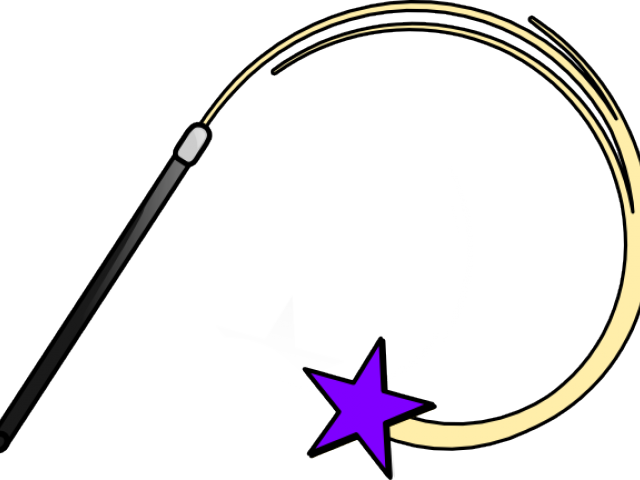
\includegraphics[width = 0.08\textwidth]{pics/wand.png}};    
\end{tikzpicture}
}
        \only<6->{\item Try to avoid local contradictions in $\Fs \rest (x = 0)$. \begin{tikzpicture}
    \node[inner sep = 0pt, xscale = -1] at (0, 0) {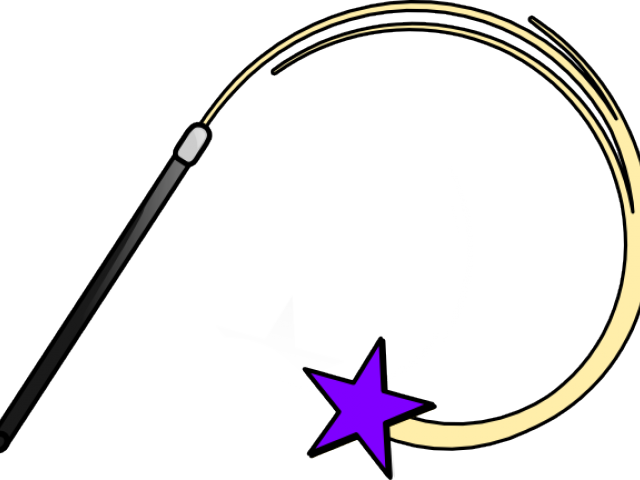
\includegraphics[width = 0.08\textwidth]{pics/wand.png}};    
\end{tikzpicture}
}
        \pause
        \pause    
        \item Repeat until we have terms of big degree.
    \end{enumerate}

    \vspace{0.3cm}
    \pause
    We kill all terms of big degree but remaining system is still hard in terms of degree.

    \vspace{0.3cm}
    \pause
    \begin{center}
        \Huge Degree is the source of hardness.
    \end{center}
\end{frame}


\begin{frame}{Degree and the $\{\pm 1\}$ basis}
    \begin{center}
        \textcolor{red}{Set $x$ to $0$ in $\pi$. This operation kills all terms that contain $x$}
    \end{center}

    \pause
    \vspace{0.5cm}

    Attempts.
    \begin{enumerate}
        \item Set $x$ to $0$. \pause \hspace{1cm} $x^2 - 1 \rest (x = 0) \to -1$.
        \pause
        \item $\tau(p) \coloneqq \frac{p \rest (x = -1) + p \rest (x = 1)}{2}$. Consider $\tau(\pi)$.
    \end{enumerate}

    \pause

    \begin{minipage}{0.3\linewidth}
        \begin{prooftree}
            \AxiomC{$p$}
            \UnaryInfC{$xp$}
            \UnaryInfC{$p$}
        \end{prooftree}
    \end{minipage}
    \pause
    \begin{minipage}{0.3\linewidth}
        \begin{prooftree}
            \AxiomC{$\tau(p)$}
            \UnaryInfC{$\tau(xp)$}
            \UnaryInfC{$\tau(p)$}
        \end{prooftree}
    \end{minipage}
    \pause
    \begin{minipage}{0.3\linewidth}
        \begin{prooftree}
            \AxiomC{$p$}
            \UnaryInfC{$0$}
            \UnaryInfC{$p$}
        \end{prooftree}
    \end{minipage}

    \pause

    Multiplication is invertible.

    \pause


    \begin{block}{Grigoriev 98; Buss, Grigoriev, Impagliazzo, Pitassi 01; Grigoriev 01}
        \begin{enumerate}
            \item Tseitin formulas has small $\PCRf[\field]$ and $\SOSf$-proofs.
            \item There are Tseitin formulas that has $\PCR[\field]$ or $\SOS$-degree $\Omega(n)$.
        \end{enumerate}
    \end{block}
\end{frame}


\begin{frame}{Degree and the $\{\pm 1\}$ basis. Part 2}

    $\pi \coloneqq (p_1, \dots, p_{\ell})$.

    Can we reduce the degree of $p_i$?
    \pause

    \begin{enumerate}
        \item $p_i \coloneqq \prod\limits_{i = 1}^{n} x_i$ \pause \hspace{0.5cm} \textcolor{green}{YES}
            \pause
            
            \begin{prooftree}
                \AxiomC{$p$}
                \UnaryInfC{$x_1 p$}
                \UnaryInfC{$\vdots$}
                \UnaryInfC{$1$}
            \end{prooftree}
            \pause
        \item $p_i \coloneqq \prod\limits_{i = 1}^{n} x_i - 1$ \pause \hspace{0.5cm} \textcolor{red}{NOT REALLY}
    \end{enumerate}

    \vspace{0.5cm}
    \pause
    $p_i \coloneqq \sum\limits_j t_j$. Degree of the symmetric differences between $t_j$'s is the new
    source of hardness.    
\end{frame}


\begin{frame}{Quadratic representation and $\Split{x}$}

    $\pi \coloneqq (p_1, \dots, p_{\ell})$.  $p_i \coloneqq \sum\limits_j t_{i, j}$.

    \pause

    $p_i^2 \coloneqq \sum\limits_{j, j'} t_{i, j} t_{i, j'}$.
    
    We want to see all possible pairs, hence we prohibit cancellations.


    \begin{block}{Quadratic representation (QR)}
        The \deftext{QR} of $\pi$ is the sequence $(p_1^2, \dots, p_{\ell}^2)$ where squares are computed
        without cancellations.
    \end{block}

    \pause
    Reminder:
    $\tau(p) \coloneqq \frac{p \rest (x = -1) + p \rest (x = 1)}{2}$.

    \pause

    We want operation that apply $\tau$ to the QR of $\pi$.

    \pause
    \begin{block}{$\Split{x}$}
        $p_i \coloneqq r_i + x q_i$.

        $\Split{x}(\pi) \coloneqq (r_1, q_1, r_2, q_2, r_3, q_3, \dots, r_{\ell}, q_{\ell})$.
    \end{block}

    \pause
    $\Split{x}(\pi)$ is a proof of \deftext{damaged} version of $\Fs$.
    
\end{frame}


\begin{frame}{Strategy for the $\{\pm 1\}$ basis ($\PCR[\field]$)}
    
    $\pi \coloneqq (p_1, \dots, p_{\ell})$ is a proof of $\Fs$. $H \coloneqq \{t \mid t \in \text{ QR of }
    \pi, \deg(t) \text{ is big}\}$.

    \begin{enumerate}
        \item $\pi$ is small $\Rightarrow$ size of $H$ is small.
        \pause
        \item Pick the most frequent literal $x$ in $H$.
        \pause
        \item Apply $\Split{x}$ to $\pi$. This operation kills all terms that contain $x$ in the QR of $\pi$.
        \pause
        \item $\Split{x}(\pi)$ is still a proof of \deftext{damaged} $\Fs$.
        \pause
        \item Try to avoid local contradictions in $\Split{x}(\Fs)$. \begin{tikzpicture}
    \node[inner sep = 0pt, xscale = -1] at (0, 0) {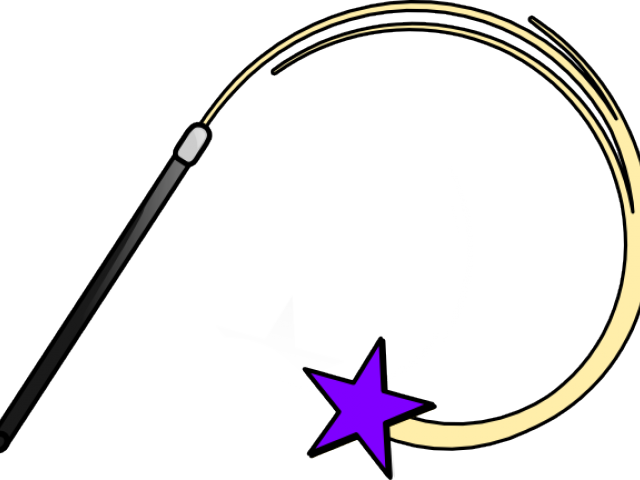
\includegraphics[width = 0.08\textwidth]{pics/wand.png}};    
\end{tikzpicture}

        \pause
        \item Repeat until we have terms of big degree in the QR.
        \vspace{0.3cm}
        \pause
        \item Try to satisfy all \deftext{broken} constraints. \pause \textcolor{red}{Impossible for
            Tseitin formulas.}
    \end{enumerate}

    \pause
    \begin{lemma}
        Let $\pi$ be a $\PCRf[\field]$-proof of $\Fs$ and QR of $\pi$ has degree $d$. Then there is a
        $\PCRf[\field]$-proof $\pi'$ of $\Fs$ of degree $2d$.
    \end{lemma}
    \pause
    \textcolor{red}{This is wrong Lemma, we need to change definition of QR to fix it.}
\end{frame}

\begin{frame}{Lazy computations}
    
    $\pi \coloneqq (p_1, \dots, p_{\ell})$ is a proof of $\Fs$.

    \pause
    \deftext{Lazy representation} of $p_i$ ($\lazy{p_i})$ in the proof $\pi$:
    \begin{itemize}
        \item $\lazy{p}_i \coloneqq p_i$, if $p_i \in \Fs$ or $p_i \coloneqq p_j$ for some $j < i$;
        \item $\lazy{p}_i \coloneqq \alpha p_j + \beta p_k$ \textcolor{blue}{without cancellations}, if
            $p_i \coloneqq \alpha p_j + \beta p_k$.
    \end{itemize}

    \pause
    The fixed \deftext{QR} of $\pi$ is the sequence $(\lazy{p}_1^2, \dots, \lazy{p}_{\ell}^2)$ where
    squares are computed without cancellations.

    \pause
    \begin{lemma}
        Let $\pi$ be a $\PCRf[\field]$-proof of $\Fs$ and QR of $\pi$ has degree $d$. Then there is a
        $\PCRf[\field]$-proof $\pi'$ of $\Fs$ of degree $2d$.
    \end{lemma}

    \pause
    $p_i \coloneqq \sum\limits_{j} t_{i, j}$ and $s_i \coloneqq \sum\limits_{j} t_{i, 1} t_{i, j}$
    \hspace{0.4cm} $\Rightarrow$ \hspace{0.4cm} $p_i = t_{i, 1} s_i$ and $s_i = t_{i, 1} p_i$.

    \pause
    $\pi'' \coloneqq (s_1, \dots, s_{\ell})$
    \pause
    
    \begin{enumerate}
        \item $\mathbf{p_i \in \boldsymbol{\Fs}}$: \hspace{0.3cm} $s_i = t_{i, 1} p_i$.
        \item $\mathbf{p_i \coloneqq x p_j}$: \hspace{0.3cm} $s_i = s_j$.
        \item $\mathbf{p_i \coloneqq \boldsymbol{\alpha} p_a + \boldsymbol{\beta} p_b}$: \hspace{0.3cm}
            \pause $q \coloneqq \alpha \sum\limits_{j} t_{a, 1} t_{a, j} + \beta \sum\limits_{j} t_{a, 1}
            t_{b, j}$.

            \pause
            $q = \alpha s_{a} +  \beta \sum\limits_{j} t_{a, 1} t_{b, j} = \alpha s_a + \beta t_{a, 1}
            t_{b, 1} \sum\limits_{j} \beta t_{b, 1} t_{b, j} = \alpha s_a + \beta t_{a, 1} t_{b, 1} s_b$.

            \pause
            $s_i = \sum\limits_{j} t_{i, 1} t_{i, j}$. Wlog $t_{i, 1} \coloneqq t_{a, k}$ hence $s_i = t_{a, k} t_{a, 1} q$.
    \end{enumerate}


\end{frame}



\begin{frame}{Open problems}

    \begin{enumerate}
        \item Lower (or upper!) bound on $\PCRf[]$-proofs of Functional Pigeonhole Principle.
        \item Lower bound on $\PCRb[]$-proofs of Weak Pigeonhole Principle.

            \begin{tikzpicture}
    \node[inner sep = 0pt] at (0, 0) {
\includegraphics[width = 0.2\textwidth]{pics/pigeon.png}};    
\end{tikzpicture}

        \pause
        \item Can we simulate Resolution in $\PCRf[\field]$? \pause Conjecture: NO.
    \end{enumerate}
\end{frame}
    \begin{frame}{Extensions}

    \pause
    \begin{block}{Open problem}
        Can we simulate Resolution in $\PCRf[]$?
    \end{block}

    \pause

    \begin{minipage}{0.48\linewidth}
        Variables:
        \begin{itemize}
            \item $x_i \in \{0, 1\}$
            \item $\bar{x}_i \coloneqq 1 - x_i$;
            \item $y_i \coloneqq 1 - 2 x_i$;
        \end{itemize}
    \end{minipage}
    \begin{minipage}{0.48\linewidth}
        Axioms:
        \begin{itemize}
            \item $x^2_i - x_i$
            \item $\bar{x}_i + x_i - 1$;
            \item $y_i + 2 x_i - 1$;
        \end{itemize}
    \end{minipage}

    \vspace{0.4cm}
    \pause

    The $\PCR[\field]_*$-proof of $\Fs$ is a sequence $(p_1, p_2, p_3, \dots, p_{\ell})$:
    \pause
    \begin{itemize}
        \item $p_i \in \Fs \cup \{\text{Axioms}\}$;
        \pause
        \item $p_i = x_j p_k$ for some $j$ and $k < i$;
        \pause    
        \item $p_i = \alpha p_k + \beta p_s$ for some $k, s < i$ and $\alpha, \beta \in \field$;
        \pause
            \item $p_{\ell} = 1$.
    \end{itemize}

    \pause
    
    $\PCR[\field]_*$ simulates $\PCRf[\field]$ and $\PCRb[\field]$.
\end{frame}


\begin{frame}{Lower bounds}
    
    \begin{theorem}
        If $\varphi$ is a random $11$-CNF formula then whp any $\PCR[\field]_*$-proof of $\varphi$ has
        size $\exp(\Omega(n))$.
    \end{theorem}


    \pause

    Can we compose techniques for the $\{0, 1\}$ and $\{\pm 1\}$ bases?

    \pause
    
    \begin{blockpic}{$\Split{x}$}{
        \node at (3, 1.8) {};
        \node[inner sep = 0pt, xscale = -1] at (0, 0)
        {
\includegraphics[width = 1.05cm]{pics/hammer.png}};
    }
    
    $p_i \coloneqq r_i + x q_i$.

    $\Split{x}(\pi) \coloneqq (r_1, q_1, r_2, q_2, r_3, q_3, \dots, r_{\ell}, q_{\ell})$.
\end{blockpic}

    $\Split{y}(y_j + 2 x_j - 1)$ \hspace{1.5cm} $\Rightarrow$ \hspace{1.5cm} $r \coloneqq 2 x_i - 1$, $q
    \coloneqq 1$.

\end{frame}


\begin{frame}{Strategy for the $\PCR[\field]_*$}

    $\pi \coloneqq (p_1, \dots, p_{\ell})$ is a proof of $\Fs$. $H \coloneqq \{t \mid t \in \text{ QR of }
    \pi, \deg(t) \text{ is big}\}$.

    \begin{enumerate}
        \item $\pi$ is small $\Rightarrow$ size of $H$ is small.
        \pause
        \item Pick the most frequent \deftext{literal} $x_i$ in $H$.
        \pause
        \item If $x_i$ is frequent then:
            \begin{itemize}
                \item set it to $0$;
                \item set $y_i$ to the right value.
            \end{itemize}
        \pause
        \item If $x_i$ is \deftext{not} frequent then:
            \begin{itemize}
                \item pick the most frequent variable $y_j$ in $H$;
                \item replace $x_j$ by $\frac{1 - y_j}{2}$;
                \item replace $\bar{x}_j$ by $\frac{1 + y_j}{2}$;
                \item expand brackets ($x_j$ and $\bar{x}_j$ are \deftext{not} frequent);
                \item apply $\Split{y_j}$ to $\pi$ set it to $0$;
            \end{itemize}
        \item Resulting proof is still a proof of \deftext{damaged} $\Fs$.
        \pause
        \item Try to avoid local contradictions in the resulting proof. \begin{tikzpicture}
    \node[inner xsep = 0pt, inner ysep = -20pt, xscale = -1] at (0, 0) {
        
\includegraphics[width = 0.27\textwidth]{pics/cat.png}
    };
    \node at (0pt, -8pt) {};
\end{tikzpicture}

        \pause
        \item Repeat until we have terms of big degree in the QR.
        \vspace{0.3cm}
        \pause
        \item Try to satisfy all \deftext{broken} constraints.
    \end{enumerate}
\end{frame}
    \begin{frame}{Open problems}

    \begin{itemize}
        \item Lower bounds for $\EQ$ dag protocols.
        \item Lower bounds for randomized dag protocols.
        \item Lower bounds NOF model of dag protocols.
        \item Can we prove the same result for constant size gadget?
    \end{itemize}

    \begin{block}{Conjecture}
        Randomized rectangle dag complexity of $S \circ \Ind_{m}$ is $n^{\Theta(w'(S))}$, where $w'(S)$ is
        width of ``random resolution refutation'' of $S$.
    \end{block}
\end{frame}
    
\end{document}
